\section{Auswertung}
\label{sec:Auswertung}

\subsection{Zum Messgerät}
\label{sub:Zum Messgerät}
  Am analogen Strommessgerät lassen sich Werte unterscheiden, bei denen die Nadel auf einen Skalenstrich oder zwischen
  zwei Skalenstriche zeigt. Entsprechend wurden alle Strommessdaten mit einem Fehler von 5\% der Skala versehen.

\subsection{Dunkelstrom}
\label{sub:Dunkelstrom}
  Zu Beginn wurde der Dunkelstrom der Diode als \SI{0.1}{\nano\ampere} gemessen. Dies liegt einige Größenordnungen unter dem durch
  den Laser erzeugten Strom und wird deswegen in der weiteren Auswertung nicht berücksichtigt.


\subsection{Spaltausmessung mit dem Mikroskop}
\label{sub:Mikroskop}
  Im weiteren sind die Spalte nach ihrer Größe absteigend durchnummeriert, der Doppelspalt trägt die Nummer vier.

  Es wurden folgende Spaltbreiten mikroskopisch bestimmt:
  \begin{table}[H]
    \centering
    \caption{Spaltparameter nach Mikroskopmessung.}
    \label{tab:innenw}
    \begin{adjustbox}{center}
    \begin{tabular}{
        S
        S
        S}
     \toprule
     \multicolumn{1}{c}{Spalt} &
     \multicolumn{1}{c}{Breite b in mm} &
     \multicolumn{1}{c}{Spaltabstand d in mm} \\
     \midrule
1 & 0.4  & n/a \\
2 & 0.16 & n/a \\
3 & 0.08 & n/a \\
4 & 0.12 & 0.48 \\
     \bottomrule
    \end{tabular}
    \end{adjustbox}
	\end{table}


\subsection{Beugungsmuster}
\label{sub:Beugungsmuster}

\begin{table}[H]
  \centering
  \caption{Fitparameter der Beugungsmuster.}
  \label{tab:fit}
  \begin{adjustbox}{center}
  \begin{tabular}{
      S
      S
      S
      S
      S
      S}
   \toprule
   \multicolumn{1}{c}{Spalt} &
   \multicolumn{1}{c}{Breite b in m} &
   \multicolumn{1}{c}{Amplitude in $\text{A}^{0.5}$} &
   \multicolumn{1}{c}{Offset in rad} &
   \multicolumn{1}{c}{Abstand d in m} &
   \multicolumn{1}{c}{Sos in $\text{A}^{2}$} \\
   \midrule
      1 & 3.57e-04 &  2.07e-01 &  1.43e-10 & n/a      & 1.5e-07 \\
      2 & 1.23e-04 &  3.51e-01 &  1.32e-04 & n/a      & 5.3e-09 \\
      3 & 5.60e-05 &  2.96e-02 & -3.36e-04 & n/a      & 1.9e-14 \\
      4 & 6.72e-05 &  9.57e-04 &  3.07e-10 & 2.37e-04 & 8.5e-08 \\
   \bottomrule
  \end{tabular}
  \end{adjustbox}
\end{table}

  Die Photodiode wurde pro Messung um jeweils \SI{0.5}{\milli\m} verschoben, vom Hauptmaximum ausgehend etwa 25 mal nach
  rechts und 25 mal nach links. Die Rohdaten mit den dazu berechneten Winkeln befinden sich im Anhang.
  Diese Daten wurden auf \ref{equ:I} bzw. \ref{equ:I_doppel} gefittet, um u.A. die Spaltbreite zu bestimmen (Tablle~\ref{tab:fit});
  dabei wurde ein Offset auf den Messwinkel addiert, um den Fit zentrieren zu können. Zudem wurde die Summer der Abweichungsquadrate
  von den Messwerten gebildet, die ein Maß für die Güte des Fits darstellen.

  Zusätzlich wurden alle Fits mit auch geplottet:

      \begin{figure}[H]
          \centering
          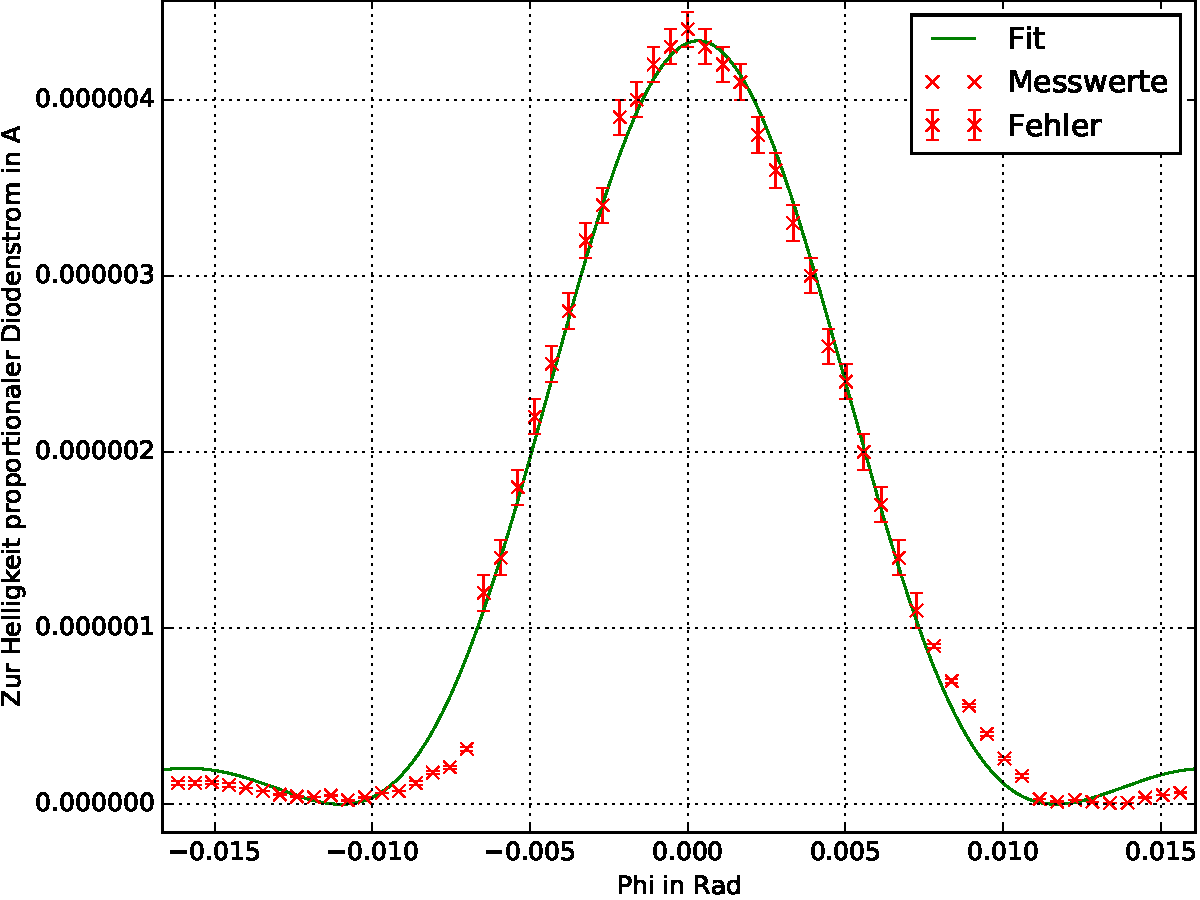
\includegraphics[width=.9\textwidth]{../plots/single_slit1.pdf}
          \caption{Großer Spalt 1}
          \label{fig:sub5}
      \end{figure}%
      
      \begin{figure}[H]
          \centering
          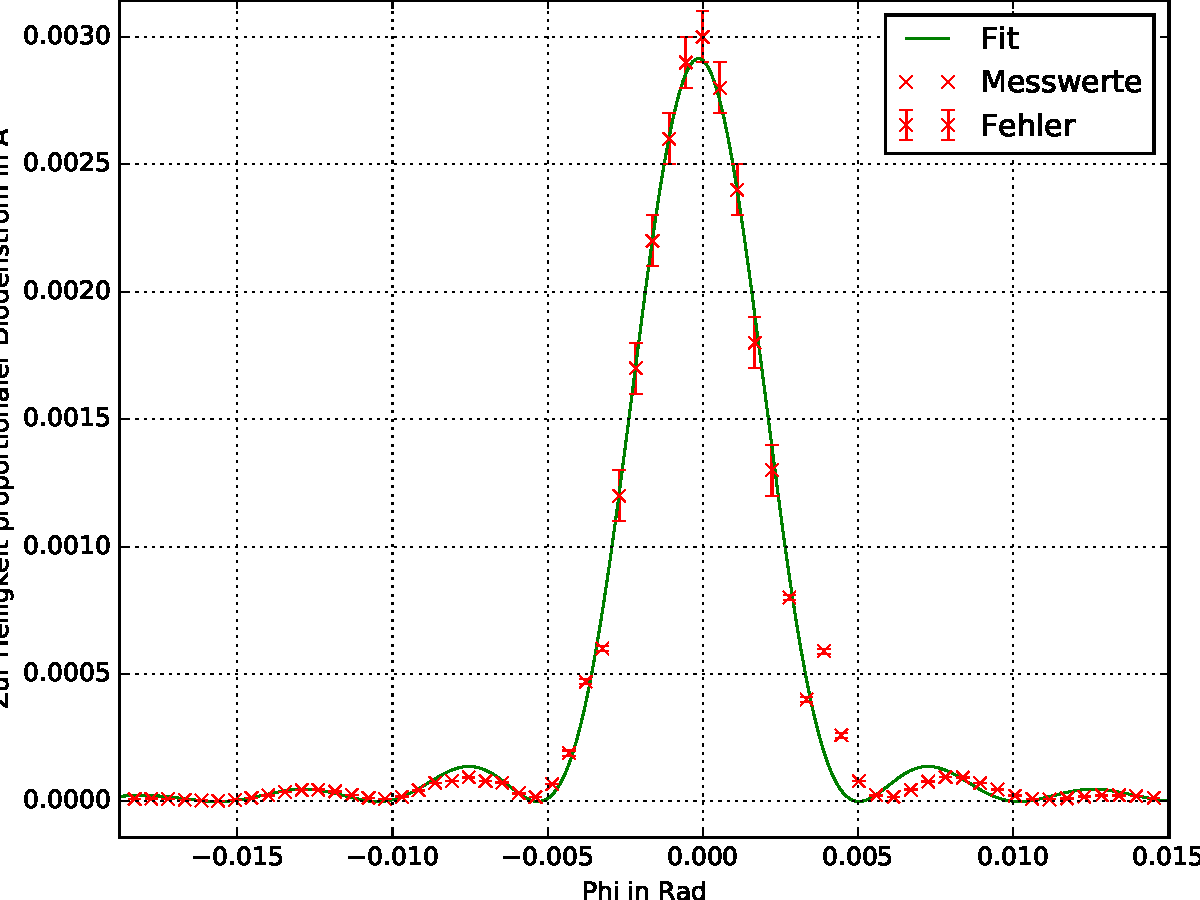
\includegraphics[width=.9\textwidth]{../plots/single_slit2.pdf}
          \caption{Mittelgroßer Spalt 2}
          \label{fig:sub4}
      \end{figure}%
      
      \begin{figure}[H]
          \centering
          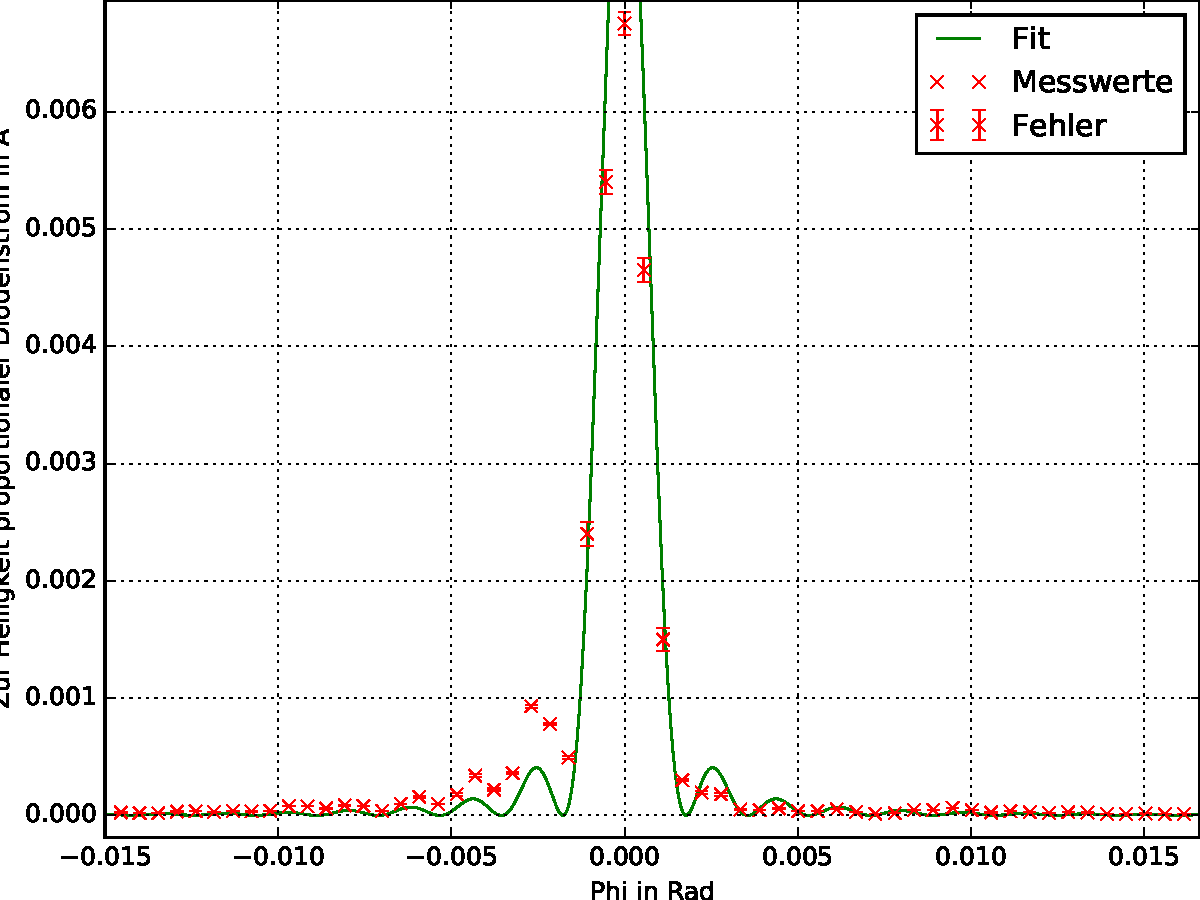
\includegraphics[width=.9\textwidth]{../plots/single_slit3.pdf}
          \caption{Kleiner Spalt 3}
          \label{fig:sub3}
      \end{figure}%
      
      \begin{figure}[H]
          \centering
          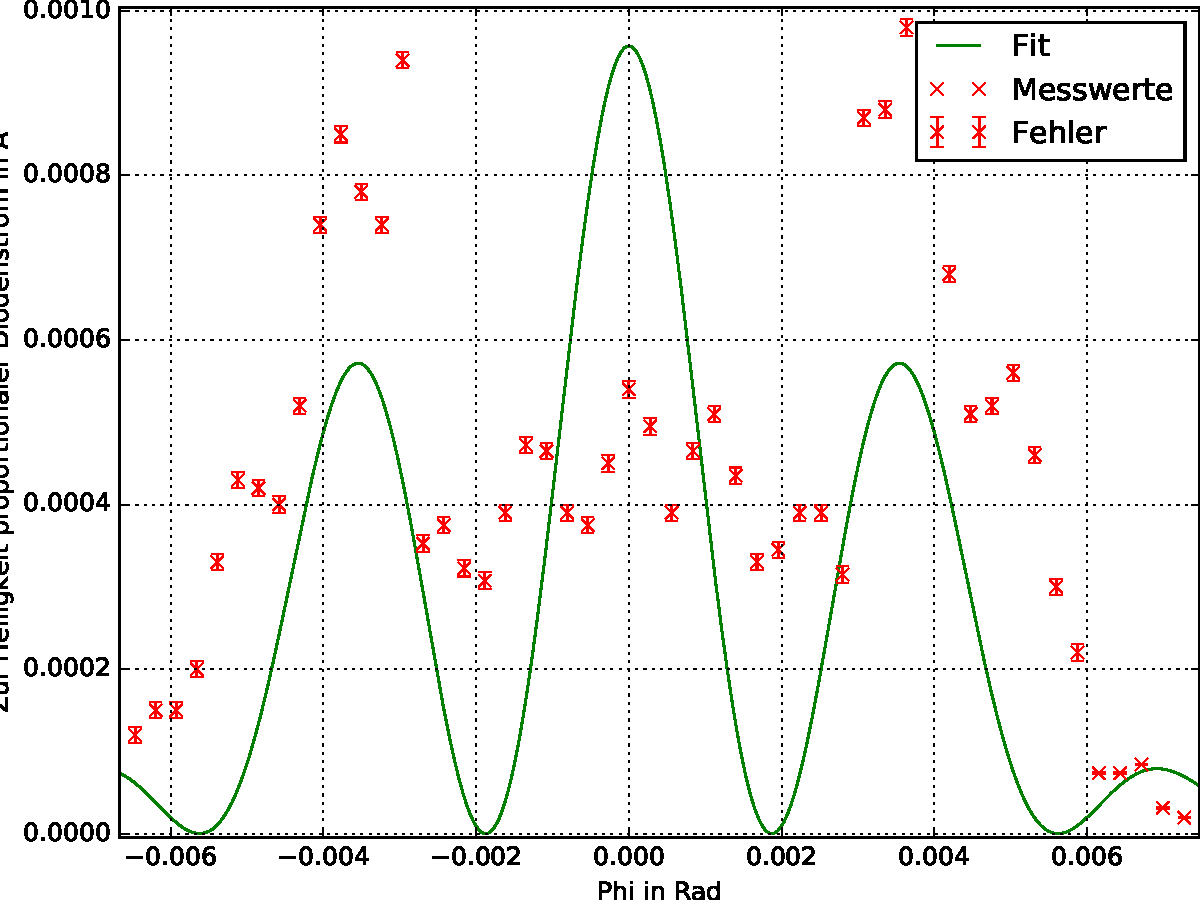
\includegraphics[width=.9\textwidth]{../plots/double_slit.pdf}
          \caption{Doppelspalt 4}
          \label{fig:sub2}
      \end{figure}%



